\documentclass[a4paper,12pt]{article}
\usepackage{fullpage}
\usepackage[T1]{fontenc}
\usepackage{amsmath}
\usepackage{amssymb}
\usepackage[utf8]{inputenc}
\usepackage{color}
\usepackage{authblk}
\usepackage{todonotes}
\usepackage{caption}
\usepackage{url}
\usepackage{float}
\usepackage{sectsty}
\usepackage{pdfpages}
\usepackage[section]{placeins}
\DeclareCaptionFont{white}{\color{white}}
\DeclareCaptionFormat{listing}{\colorbox{gray}{\parbox{\textwidth}{#1#2#3}}}
\captionsetup[lstlisting]{format=listing,labelfont=white,textfont=white}

\usepackage{setspace}
\usepackage[toc,page]{appendix}
\usepackage{framed}
\usepackage{geometry}

\usepackage{alltt}
\usepackage{subfig}

% Change section fonts
\allsectionsfont{\sffamily}

% For code box
\usepackage{xcolor}
\usepackage{listings}
\usepackage{caption}
\DeclareCaptionFont{white}{\color{white}}
\DeclareCaptionFormat{listing}{%
  \parbox{\textwidth}{\colorbox{gray}{\parbox{\textwidth}{#1#2#3}}\vskip-4pt}}
  \captionsetup[lstlisting]{format=listing,labelfont=white,textfont=white}
  \lstset{frame=lrb,xleftmargin=\fboxsep,xrightmargin=-\fboxsep}
% End code box

\usepackage{cite}

% General parameters, for ALL pages:
\renewcommand{\topfraction}{0.9}	% max fraction of floats at top
\renewcommand{\bottomfraction}{0.8}	% max fraction of floats at bottom
% Parameters for TEXT pages (not float pages):
\setcounter{topnumber}{2}
\setcounter{bottomnumber}{2}
\setcounter{totalnumber}{4} % 2 may work better
\setcounter{dbltopnumber}{2} % for 2-column pages

\addtolength{\topmargin}{0.5in}

\usepackage{fancyvrb}

\usepackage{tikz} \usetikzlibrary{trees}
\usepackage{hyperref} % should always be the last package

% useful colours (use sparingly!):
\newcommand{\blue}[1]{{\color{blue}#1}}
\newcommand{\green}[1]{{\color{green}#1}}
\newcommand{\red}[1]{{\color{red}#1}}

% useful wrappers for algorithmic/Python notation:
\newcommand{\length}[1]{\text{len}(#1)}
\newcommand{\twodots}{\mathinner{\ldotp\ldotp}} % taken from clrscode3e.sty
\newcommand{\Oh}[1]{\mathcal{O}\left(#1\right)}

% useful (wrappers for) math symbols:
\newcommand{\Cardinality}[1]{\left\lvert#1\right\rvert}
\newcommand{\Ceiling}[1]{\left\lceil#1\right\rceil}
\newcommand{\Floor}[1]{\left\lfloor#1\right\rfloor}
\newcommand{\Iff}{\Leftrightarrow}
\newcommand{\Implies}{\Rightarrow}
\newcommand{\Intersect}{\cap}
\newcommand{\Sequence}[1]{\left[#1\right]}
\newcommand{\Set}[1]{\left\{#1\right\}}
\newcommand{\SetComp}[2]{\Set{#1\SuchThat#2}}
\newcommand{\SuchThat}{\mid}
\newcommand{\Tuple}[1]{\langle#1\rangle}
\newcommand{\Union}{\cup}
\usetikzlibrary{positioning,shapes,shadows,arrows}
\providecommand{\keywords}[1]{\textbf{\textit{Keywords: }} #1}

\title{\textbf{Designing a Virtual Security Layer for Cloud Content}}
\author{Lukas Klingsbo}

\begin{document}

\maketitle
%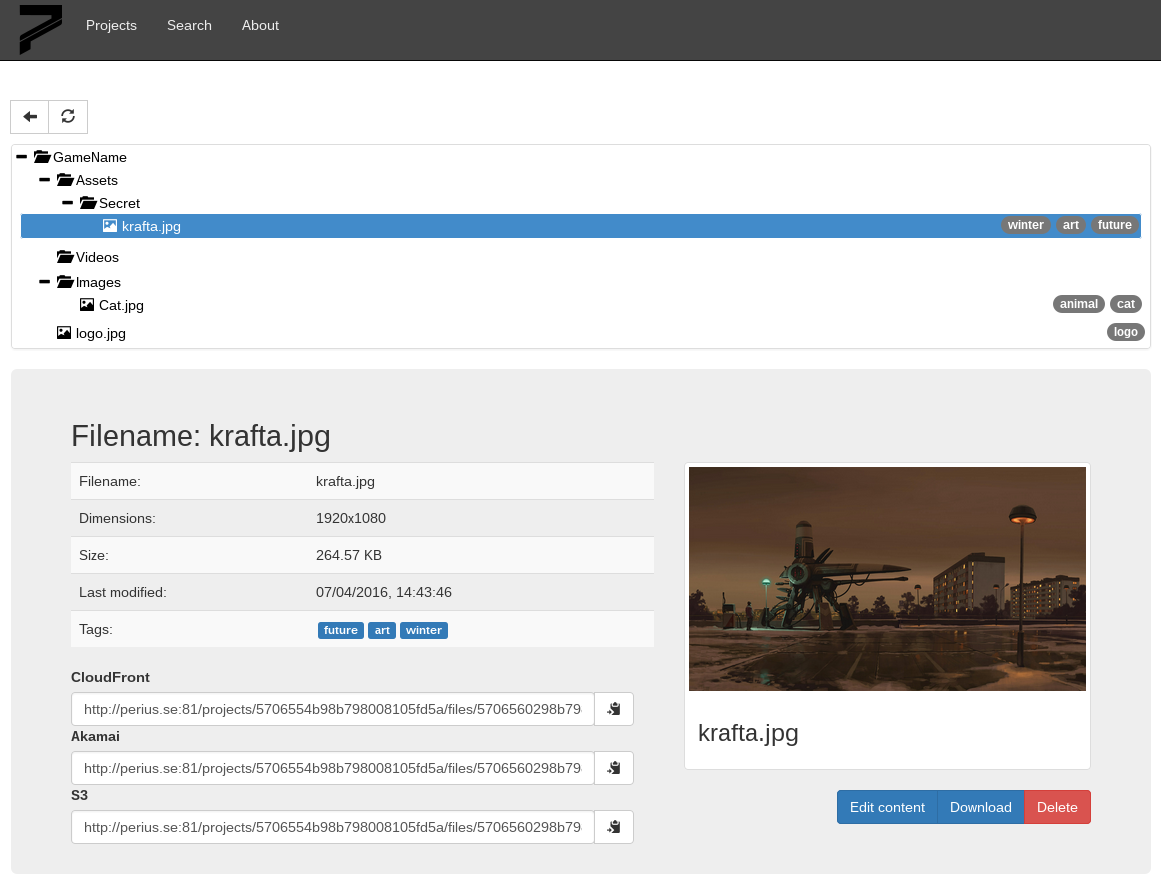
\includepdf[pages={1}]{front.pdf}
%\thispagestyle{empty}
%\newpage\null\thispagestyle{empty}\newpage

\pagenumbering{roman}
\setcounter{page}{2}

%\includepdf[pages={1}]{abstract.pdf}
\begin{abstract}
    TODO: Abstract

\keywords{}
\end{abstract}

\newpage\null\thispagestyle{empty}\newpage

\setcounter{tocdepth}{3}
\tableofcontents

\clearpage
\pagenumbering{arabic}
\setcounter{page}{1}
\section{Introduction}
Developing larger projects containing static content usually involves using a Content Distribution Network 
to be able to scale to a large user base. The commercial Content Distribution Networks are usually fairly easy to use, 
the content that is to be used in a project is usually simply uploaded and then directly available to the public. 
For secret content this can be a problem and that is what this thesis is about. This work examines ways of enforcing 
access control on content and groups of content in the form of snapshots. A system was developed to make the underlying 
theory work in practice. 

\newpage
\section{Related Terminology}
\subsection{Technologies}
\subsubsection{React}
React is a JavaScript library for building user interfaces. React uses both its own virtual DOM and the browser's, 
this makes it able to efficiently update dynamic web pages after a change of state through comparing the old virtual 
DOM with the resulting virtual DOM after the state change and then only update the browser's DOM according to the 
difference between the virtual DOMs~\cite{REACT}.

\subsubsection{Flux}


\subsubsection{Scala}
Scala is a multi-paradigm programming language. It most commonly runs on the JVM and compared to Java it supports 
most functional programming features at the same time as it supports object oriented programming~\cite{SCALA}.

\subsubsection{REST}
\subsubsection{MongoDB}
    TODO: Write down related terminology, if any
\subsection{Abbreviations}

\subsubsection{JPF}
Java Path Finder - It was developed by NASA and in 2005 they released it under an open source licence, which made more 
people contribute to the project. JPF is usually used for doing model checking of concurrent programs to easily find 
for example race conditions and dead locks.

\subsubsection{CDN}
Content Distribution/Delivery Network - Replicates content to several servers, usually spread out geographically. Once a 
request is made, the network serves content from the server closest to the requester.

\section{Related Work}
\subsection{Copy-on-Write}
This work relies heavily on the Copy-on-Write principle which was founded and used in the Mach kernel~\cite{COPYONWRITE}. 

Copy-on-Write is used in virtual memory management systems~\cite{VIRTCOW}, snapshot functionality in both file 
systems~\cite{FSCOW} and logical volume management systems~\cite{LVMCOW}, and as an optimisation technique for objects and 
types in programming languages\cite{LANGCOW}.

Its principle is that when processes share data in between each other, the data is not copied until one of the processes 
does changes to it. This is an optimisation as the processes does not have to send all of the related data that is in memory, 
rather they only have to send pointers to the data. After many Copy-on-Write's a complex structure can be built up, 
but it is possible to solve that structure~\cite{COPYONWRITE2}.



\section{Background}
\subsection{About Uprise}
Uprise is a company based in Uppsala, Sweden. 

\subsection{The current system}
Today a system called battlebinary~\cite{BATTLEBINARY} is used for managing and uploading files, mostly images, to content 
delivery networks. The current system does not make use out of the security features that the CDN's are offering, instead it 
uses a form of security by obscurity. When a file is uploaded to a CDN it is open for the public, but its filename is 
composed out of its original filename concatenated with a part of the MD5 hash of the content of the file, which makes it an 
extremely hard process to access the file on the CDN without access to the original file or a reference to the URI.

In the current system you can only upload a file once as there will be a collision in the upload otherwise, as the old and 
the new file will have the same MD5 hash.  

\subsection{Problem description}
As the current system does not offer proper security measurements, is lacking a lot of features that is needed and does not 
scale very well, a new system should be developed. This work is about examining a way of implementing Copy-on-Write in a 
high level system, which should solve the scalability problem and makes it possible to implement the wanted features, like 
snapshots and concurrent modifications of content.

What to write about
Battle Binary
Security features of CDN's

What is needed
* Security layers
* snapshots
* Virtual file structure
* Versioning of content
* Multi project support
* Auth and audit logs
* Users
\newpage 
\section{Model}
\subsection{Entities}
%\subsubsection*{snapshot} for not having section numbers
\begin{figure}[htp] \centering{
    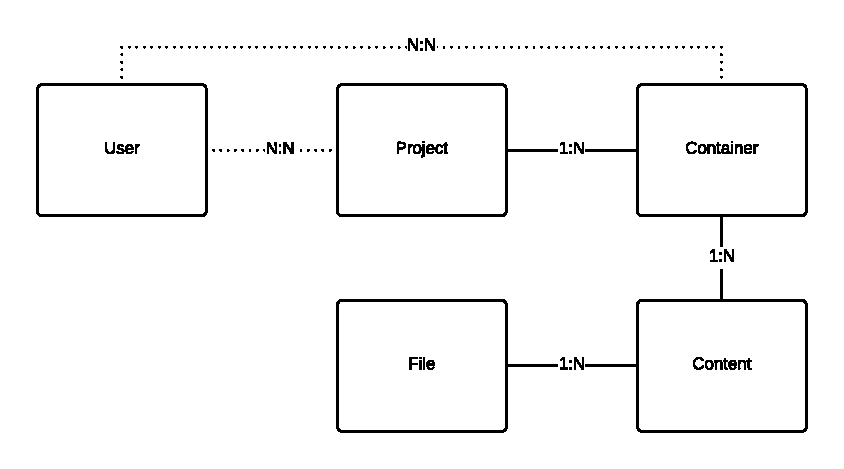
\includegraphics[scale=0.8]{relation.pdf}}
    \caption{Entity Relationships}
    \label{fig:relation}
\end{figure}

\subsubsection{Content}
Content is an asset contained in a project and/or snapshot, it is a form of virtual file.
It could be described as a link between the snapshot or project and the real file. 
The content can be for example an image, video or binary blob, combined with meta-data.

\subsubsection{Project}
A project is what is created to contain all content related to a real project. Files can be changed within a project and 
the system can contain several projects and their virtual content are completely disjoint.
snapshot
\subsubsection{Snapshot}
A snapshot is a read-only container from the state which the container the was in when the snapshot was created. A snapshot can 
have content which either is automatically dependant on the container which it was created from and updated when that container 
is updated or stay in the state which it was in when the snapshot was created. This results in that the content within a snapshot 
can not be updated independently from the container which it was created from.

\subsubsection{Container}
A container is a virtual folder within the projects which contains content and other containers.

\subsubsection{File}
A file refers to an actual physical file in the file system.

\subsubsection{User}
A user is the structure that handles people who have been granted access to the system.
Access to the system is handled by a separate service, like LDAP.

\subsection{JPF}
Java path finder was used to show that the model and plan of how to build the system was sound. The model was built in Java 
with the objective of being as reduced and simple as possible, without loosing any of the cases that needs to be covered 
by the model checker. As the users are mainly going to be handled by external systems they were not included in the model.

Each collection in the persistent storage was emulated by using the built-in ConcurrentHashMap type. 
Each client was represented by a thread and each action taken by the client was randomised. The id hashes which MongoDB is 
using for each entity was imported from the mongo-java-driver-2.13.3 and each object had its own id, generated in the same 
fashion as the real implementation is using, randomly generated by the ObjectId class to minimise collisions that is. 
Further more no locking or transactions were used and the threads were running fully concurrently, without any sleep statements. 

ConcurrentHashMap had to be used in favour of the normal HashMap as the normal HashMaps can't be iterated over concurrently.

JPF checked each permutation of states that the threads can end up in, the result of the run can be seen in Listing~\ref{JPFRESULT}.

\begin{lstlisting}[label=JPFRESULT,caption=Results of JPF run]
elapsed time:       14:26:53
states:             new=160853259,
                    visited=451102505,
                    backtracked=611955764,
                    end=21640
search:             maxDepth=380,
                    constraints=0
choice generators:  thread=160853255 
                    (signal=0,
                    lock=3603938,
                    sharedRef=146989208,
                    threadApi=3,
                    reschedule=10260106), 
                    data=0

heap:               new=676056850,
                    released=435060996,
                    maxLive=655,
                    gcCycles=523950061

instructions:       11917045758
max memory:         6256MB
loaded code:        classes=111,
                    methods=2179
\end{lstlisting}

\newpage 
\section{Copy-on-Write}
As the persistent storage does not implement transactions or locks a lot of different problems can occur when several 
clients are working on the same data set at the same time. Such problems could be race conditions, 

\section{Methods for determining\\implementation details}
This chapter introduces the different methods used to determine how the new system should be implemented, 
which DBMS it should use and how the estimation of long term scaling was done.

\section{Security of the system}
\subsection{Authorization}
\subsection{Audit logs}


\section{Resulting system}
\subsection{Persistent storage}
\subsubsection{MongoDB}
MongoDB was chosen as the persistent storage because of its internal storage format called BSON, which is very similar to JSON 
which the API is using. As the formats are similar, the process of marshalling and unmarshalling becomes quite easy between 
the core code, MongoDB instance and REST interface. The second reason was that if the system needs to scale in the future it 
is very easy to distribute MongoDB and if needed the system can easily be migrated to Reactive Mongo, which is asynchronous and 
non-blocking and can therefore scale even further~\cite{REACTIVEMONGO}.

\subsection{API}
REST was chosen as the BSON format which is used in MongoDB is almost identical ~\cite{BSON} to the standardised JSON 
format which is used by RESTful services~\cite{JSON}. 

\subsubsection{REST Endpoints}
For the frontend to communicate with the backend REST is used, the following endpoints were configured:

\begin{itemize}
  \item projects
      \subitem GET - list all projects
      \subitem POST - create new project
  \item projects/\{id\}
      \subitem GET - get specific project
      \subitem PUT - update existing project
      \subitem DELETE - delete existing project
  \item projects/\{id\}/content
      \subitem GET - list all content in a specific project
      \subitem POST - create new content in a specific project 
  \item projects/\{id\}/content/\{id\}
      \subitem GET - get specific content in a specific project
      \subitem PUT - update existing content in a specific project
      \subitem DELETE - delete existing content in a specific project

  \item projects/\{id\}/snapshots
      \subitem GET - list all snapshots in a specific project
      \subitem POST - create new snapshot in a specific project 
  \item projects/\{id\}/snapshots/\{id\}
      \subitem GET - get specific snapshot in a specific project
      \subitem PUT - update existing snapshot
      \subitem DELETE - delete existing snapshot
  \item projects/\{id\}/snapshots/\{id\}/content
      \subitem GET - list all content in a specific snapshot
      \subitem POST - create new content in a specific snapshot 
  \item projects/\{id\}/snapshots/\{id\}/content/\{id\}
      \subitem GET - get specific content in a specific snapshot
      \subitem PUT - update existing content in a specific snapshot
      \subitem DELETE - delete existing content in a specific snapshot

  \item projects/\{id\}/containers
      \subitem GET - list all containers in a specific project
      \subitem POST - create new container in a specific project 
  \item projects/\{id\}/containers/\{id\}
      \subitem GET - get specific container in a specific project
      \subitem PUT - update existing container
      \subitem DELETE - delete existing container
  \item projects/\{id\}/containers/\{id\}/content
      \subitem GET - list all content in a specific container
      \subitem POST - create new content in a specific container 
  \item projects/\{id\}/containers/\{id\}/content/\{id\}
      \subitem GET - get specific content in a specific container
      \subitem PUT - update existing content in a specific container
      \subitem DELETE - delete existing content in a specific container
\end{itemize}

\subsection{Scalability}

\section{Discussion}

\section{Summary}
\subsection{Conclusions}

\subsection{Future work}

Stuff to write about:
Modular design, every piece should be interchangable
LDAP - why it was used as standard AUTH


\newpage
\bibliographystyle{ieeetr}
\bibliography{references}

\end{document}
